\section{SubQuery}
\hrulefill

\begin{itemize}
    \item Retrieve the managers associated with teams established before a specific date
\end{itemize}

\begin{lstlisting}[caption={ Query 1},label={lst:q-1}]
    SELECT Manager_Name
    FROM Manager
    WHERE Manager_ID IN (
        SELECT Manager_ID
        FROM Team
        WHERE Team_Established_Date < TO_DATE('2022-03-01', 'YYYY-MM-DD')
);
\end{lstlisting}

\begin{figure}[H]
    \centering
    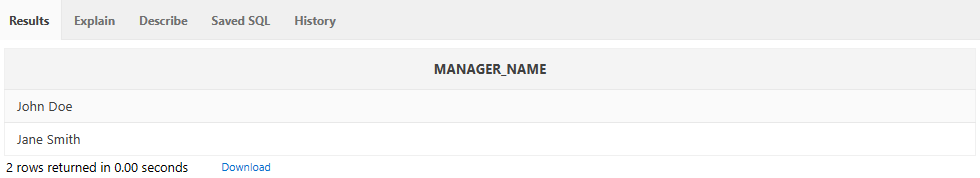
\includegraphics[width=1\textwidth]{images/dml/Subq/q1.png}
    \caption{Result of Query 1}
\end{figure}
%%%
\vspace{2cm}
\begin{itemize}
    \item Get the content creators who have a higher salary than the average salary of all content creators
\end{itemize}
\begin{lstlisting}[caption={ Query 2},label={lst:q-2}]
    SELECT ContentCreator_Name
    FROM ContentCreator
    WHERE ContentCreator_Salary > (
        SELECT AVG(ContentCreator_Salary)
        FROM ContentCreator
    );    
\end{lstlisting}
\begin{figure}[H]
    \centering
    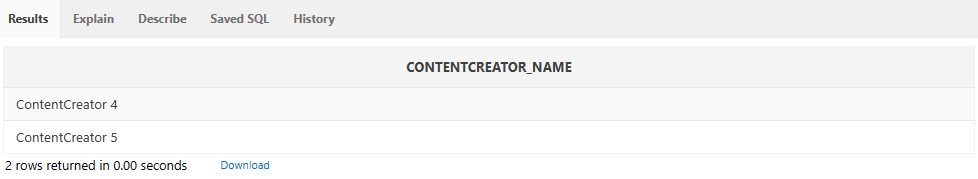
\includegraphics[width=1\textwidth]{images/dml/Subq/q2.png}
    \caption{Result of Query 2}
\end{figure}
%%% 
\clearpage
\begin{itemize}
    \item Retrieve the teams managed by managers who have won a championship
\end{itemize}
\begin{lstlisting}[caption={ Query 3},label={lst:q-3}]
    SELECT Team_Name
    FROM Team
    WHERE Manager_ID IN (
    SELECT Manager_ID
    FROM Manager
    WHERE Manager_ID IN (
        SELECT DISTINCT Manager_ID
        FROM Team_Winning
        WHERE Team_Winning LIKE '%Championship%'
    )
);
\end{lstlisting}
\begin{figure}[H]
    \centering
    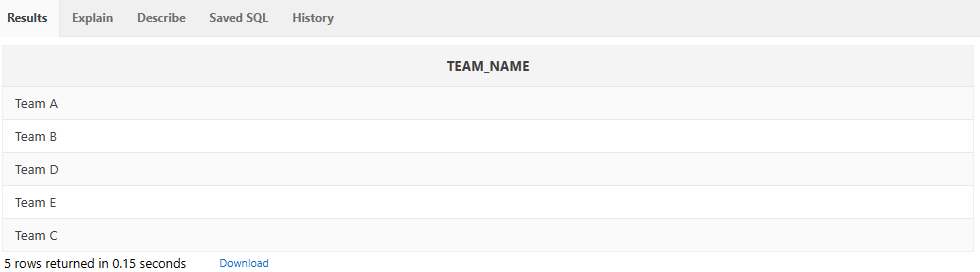
\includegraphics[width=1\textwidth]{images/dml/Subq/q3.png}
    \caption{Result of Query 3}
\end{figure}
\clearpage